\documentclass[]{article}

\usepackage{array}
\usepackage{mdwmath}
\usepackage{mdwtab}
\usepackage{eqparbox}
\usepackage[caption=false,font=footnotesize]{subfig}
\usepackage{fixltx2e}
\usepackage{stfloats}
\usepackage{url}
\usepackage{authblk}

\usepackage[utf8]{inputenc}
\usepackage{times}
\usepackage{amssymb,amsfonts,amsmath,amscd}
\usepackage[pdftex]{hyperref}
\usepackage[pdftex]{graphicx}
\usepackage{fnpos}
\usepackage{multicol}
\usepackage{multirow}
\usepackage{wasysym}
\usepackage{enumerate}
\usepackage{enumitem}
\usepackage{tikz}
\usetikzlibrary{calc}
\usepackage{pgfplots}
\usepackage{listings}
\usepackage{framed}
\usepackage{courier}
\setcounter{MaxMatrixCols}{20}
\usepackage{epsfig}
\usepackage{comment}
\usepackage[space]{cite}

\bibliographystyle{plain}
\DeclareGraphicsExtensions{.pdf,.jpeg,.png,.eps}
\graphicspath{{figures/}}

% General page formatting
\vfuzz2pt
\hfuzz2pt
\addtolength{\hoffset}{-0.8in} \addtolength{\voffset}{-0.75in}
\setlength{\textwidth}{6.7in} \setlength{\textheight}{8.25in}
\setlength{\headheight}{0.6in}
\setlength{\headsep}{0.55in}
\setlength{\footskip}{40pt}
\setlength{\fboxsep}{12pt}
\setlength{\parskip}{3pt}
\makeFNbottom \makeFNbelow
\setcounter{MaxMatrixCols}{20}

% Math definitions
\newcommand{\norm}[1]{\left\Vert#1\right\Vert}
\newcommand{\abs}[1]{\left\vert#1\right\vert}
\newcommand{\set}[1]{\left\{#1\right\}}
\newcommand{\To}{\longrightarrow}
\newcommand{\Ker}{\textup{Ker}}
\newcommand{\Img}{\textup{Img}}
\newcommand{\diag}{\textup{diag}}
\newcommand{\circulant}{\textup{circ}}
\newcommand{\bcf}{\;\mbox{\boldmath ${\cal F}$\unboldmath}}
\def\Vec#1{\!\!\hbox{$#1$\kern-0.38em\lower0.85em\hbox{$\vec{}\,$}}\,}%
\newcommand{\bbm}{\begin{bmatrix}}
\newcommand{\ebm}{\end{bmatrix}}
\newcommand{\mbf}[1]{\mathbf{#1}}
\newcommand{\mbs}[1]{{\boldsymbol{#1}}}
\newcommand{\mbb}[1]{{\mathbb{#1}}}
\newcommand{\mc}[1]{\mathcal{#1}}
\newcommand{\argmin}{\operatornamewithlimits{argmin}}
\newcommand{\argmax}{\operatornamewithlimits{argmax}}
\newcommand{\expect}{\operatornamewithlimits{\mbb{E}}}

\begin{document}

\title{Robostats Lab 1 \\ Particle Filtering}
\author{Vishnu Desaraju}
\author{John Yao}
\affil{The Robotics Institute, Carnegie Mellon University\\ \{rajeswar, johnyao\}@cmu.edu}

\maketitle

\section{Approach}

\subsection{Notation}

\begin{tabular}{ c p{13.5cm} }
  \textbf{Symbol} & \textbf{Meaning} \\ \hline
        $\mbf{x}$ & robot state (position and heading in world frame) \\
        $\mbf{z}$ & vector of 180 laser range returns \\
        $\mbf{m}$ & the map \\
     $(x_r, y_r)$ & robot position in world frame \\
     $\psi_r$ & robot heading in world frame \\
           $n$ & additive Gaussian noise \\
 $\mathcal{N}(\mu, \sigma^2)$ & Gaussian distribution with mean $\mu$ and variance $\sigma$ \\
                   $\theta_i$ & laser beam heading angle relative to the robot body +$x$ axis, $\theta_1 \approx -\frac{\pi}{2}$, $\theta_{180} \approx \frac{\pi}{2}$
\end{tabular}

\subsection{Initialization}
The particles are uniformly distributed across the regions of the map that have an occupancy probability lower than a user-defined threshold.
All particle weights are initially equal.

\subsection{Motion Model}
\label{sec:motion_model}
An odometry measurement represents the incremental motion of the robot from $t_k$ to $t_{k+1}$, expressed in the robot body frame at $t_k$.
This incremental motion can be decomposed into a linear component parallel to the heading ($\Delta x$), a linear component perpendicular to the heading ($\Delta y$), and a change in the heading ($\Delta \psi$).
We assume that each component of the odometry measurement is corrupted by additive zero-mean Gaussian noise.
\begin{align}
  n_{\Delta x} &= \mathcal{N}(0, \sigma_{\Delta x}^2 ) \\
  n_{\Delta y} &= \mathcal{N}(0, \sigma_{\Delta y}^2 ) \\
  n_{\Delta \psi} &= \mathcal{N}(0, \sigma_{\Delta \psi}^2 )
\end{align}
The update equations for the robot state are:
\begin{align}
  x_{r,k+1} &= x_{r,k} + \cos \psi_{r,k} \cdot \Delta x - \sin \psi_{r,k} \cdot \Delta y + n_{\Delta x} \\
  y_{r,k+1} &= y_{r,k} + \sin \psi_{r,k} \cdot \Delta x + \sin \psi_{r,k} \cdot \Delta y + n_{\Delta y} \\
  \psi_{r,k+1} &= \psi_{r,k+1} + \Delta \psi + n_{\Delta \psi}
\end{align}

\subsection{Sensor Model}
\label{sec:sensor_model}
The sensor model describes the distribution $P(\mbf{z} | \mbf{x})$.
We first assume for simplicity that the distribution of each individual laser range return is independent (not true in real life).
\begin{align}
  P(\mbf{z} | \mbf{x}) &= \prod_{i=1}^{180} P(z_i | \mbf{x}) \label{eq:pzx_indep}
\end{align}
We also assume that each of the individual range return distributions is a Gaussian with mean $h(\mbf{x},\theta_i, \mbf{m})$ and variance $\sigma_\text{hit}^2$.
The range prediction $h$ is computed by ray tracing along the world frame heading $\psi_r + \theta_i$ from a location $25$ cm in front of the robot until hitting an occupied grid cell or an unknown grid cell.
In the former case, $h$ is the accumulated range, while in the latter case, $h$ is assigned a random value uniformly distributed between the accumulated range and the max range.


\subsection{Resampling}
In the importance resampling step, we replace the current set of particles with a new set of particles sampled from a distribution where the probability of selecting a particle is proportional to its weight, $P(\mbf{z} | \mbf{x})$.

\section{Implementation}

\subsection{Data Parsing}
Since all the provided odometry data is expressed in the same arbitrary reference frame, 2D pose differencing is required to extract the measurements required by the motion model (Section \ref{sec:motion_model}).
Suppose we have two consecutive pose readings (expressed in the same frame) at timestep $k-1$ and $k$.
The incremental pose associated with an odometry measurement at $t_k$ is
\begin{align}
  \bbm  \Delta x \\ \Delta y \ebm &= \bbm \cos \psi_{k-1} & \sin \psi_{k-1} \\ -\sin \psi_{k-1} & \cos \psi_{k-1} \ebm \bbm x_k - x_{k-1} \\ y_k - y_{k-1} \ebm \\
                      \Delta \psi &= \texttt{shortest\_angular\_distance}(\psi_k, \psi_{k-1})
\end{align}


\subsection{Log Weights to Prevent Numerical Overflow}
The straightforward description of the particle filter algorithm in \cite{thrun2005probabilistic} cannot be implemented as-is due to problems with numerical overflow when working with extremely small probabilities, which will arise in \eqref{eq:pzx_indep}.
Instead of keeping track of particle weights, we keep track of the log weights.
Then \eqref{eq:pzx_indep} becomes
\begin{align}
  \log P(\mbf{z} | \mbf{x}) &= \sum_{i=1}^{180} \log P(z_i | \mbf{x}) \\
  \log P(\mbf{z} | \mbf{x}) &= - \sum_{i=1}^{180} \frac{\left( z_i - h(\mbf{x}, \theta_i, \mbf{x}) \right)^2}{\sigma_{\text{hit}}^2}
\end{align}
Normalization of log weights can be done by subtracting the log of the sum of all regular weights from each particle's log weight.

\subsection{Parameter Tuning}
Number of particles

$\sigma_{\Delta x}$, $\sigma_{\Delta y}$, $\sigma_{\Delta \psi}$

$\sigma_\text{hit}$

cell full and empty probability thresholds

laser max range

\section{Results}

\subsection{Dataset 1: \texttt{robotdata1.log}}

Figure~\ref{fig:Screenshot-video_log1-10k_good} shows snapshots from a run using the first data log. The particles start spread across the map but are able to converge to a single cluster in a reasonable amount of time. The motion of this cluster, including changing directions twice in the hallway and ending in the room, is consistent with \texttt{robotmovie1.gif}, indicating the particle filter was able to accurately localize the robot. Total runtime was around 25 minutes.\\ Video is available here: \url{https://www.youtube.com/watch?v=DxhAmjijvzI}

\begin{figure}[h]
\centering
\begin{subfigure}[b]{0.49\textwidth}
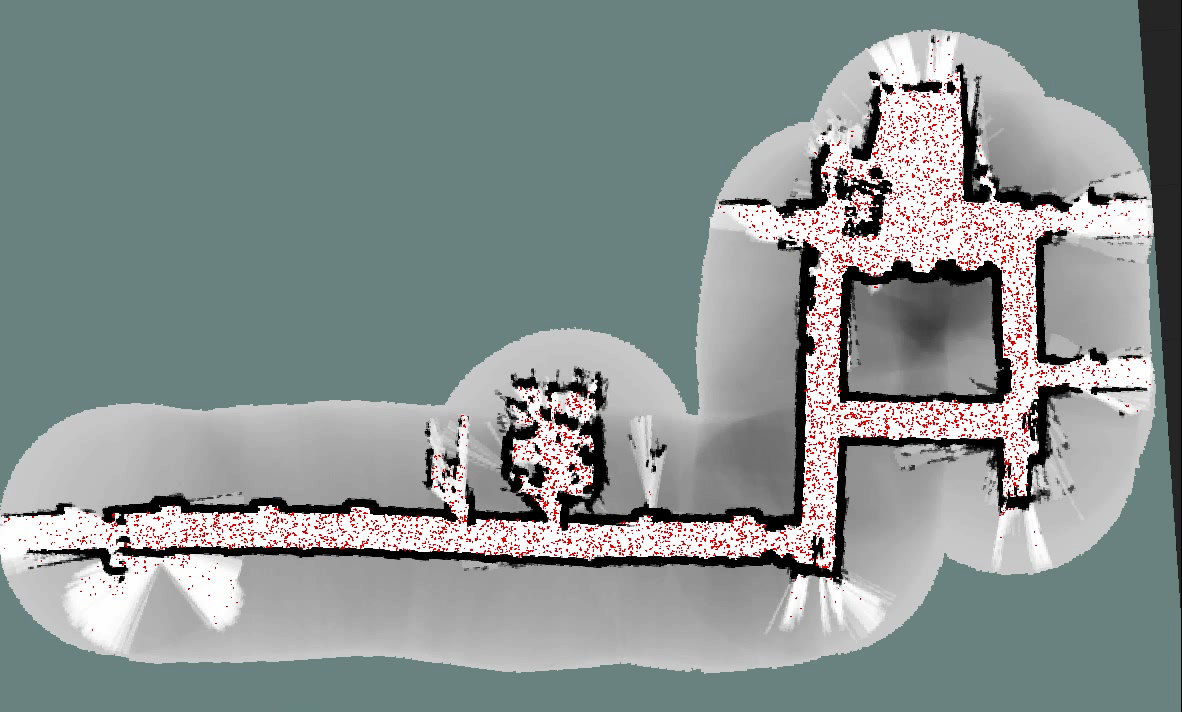
\includegraphics[width=\linewidth]{figures/Screenshot-video_log1-10k_good-1}
\caption{Initial distribution of particles}
\label{fig:Screenshot-video_log1-10k_good-1}
\end{subfigure}
\begin{subfigure}[b]{0.49\textwidth}
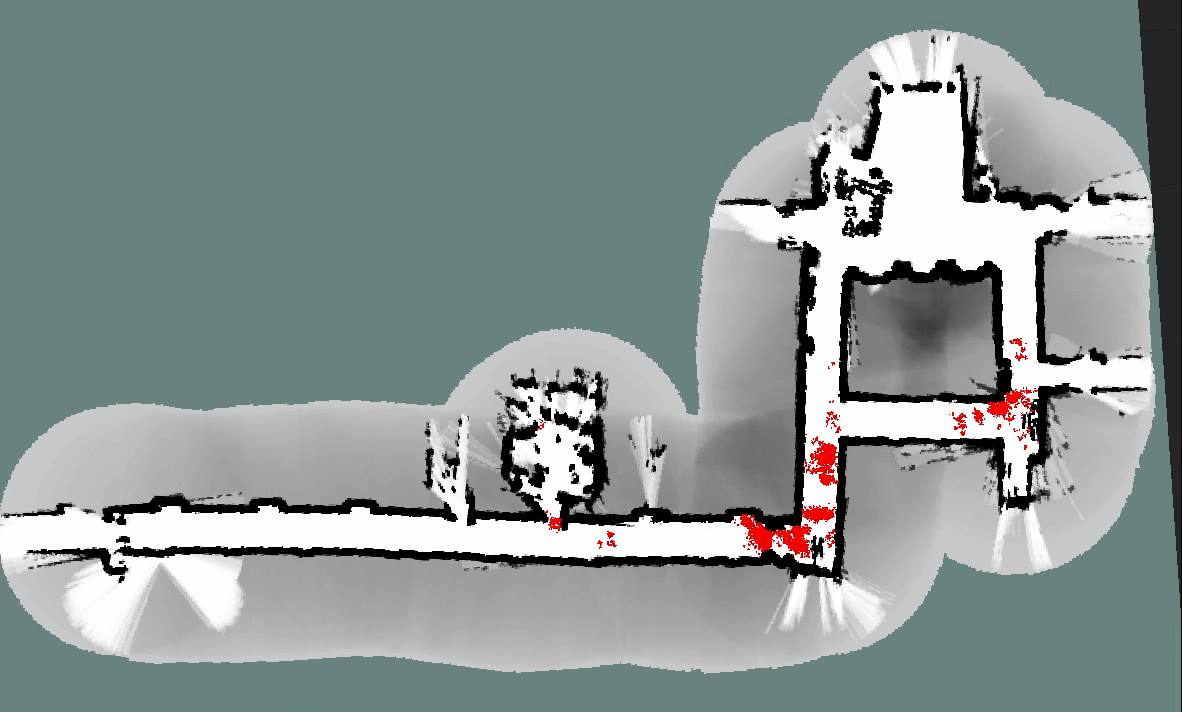
\includegraphics[width=\linewidth]{figures/Screenshot-video_log1-10k_good-2}
\caption{Particles start to converge}
\label{fig:Screenshot-video_log1-10k_good-2}
\end{subfigure}
\\
\begin{subfigure}[b]{0.49\textwidth}
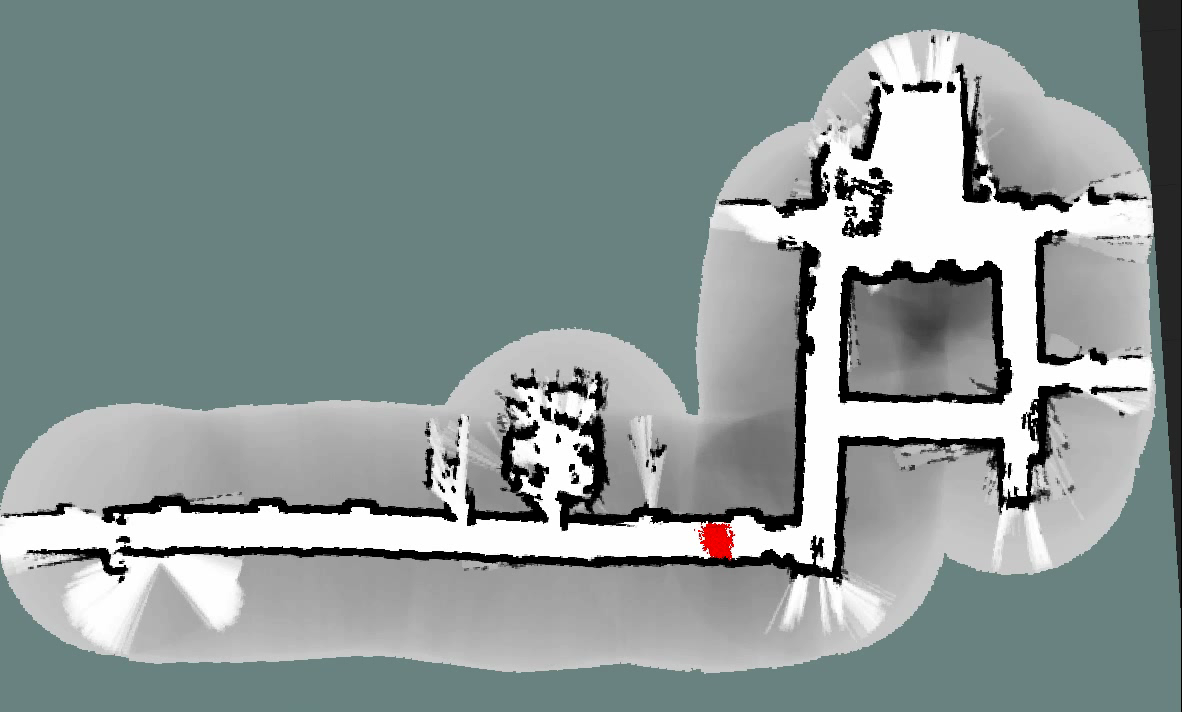
\includegraphics[width=\linewidth]{figures/Screenshot-video_log1-10k_good-3}
\caption{Particles have converged to one location}
\label{fig:Screenshot-video_log1-10k_good-3}
\end{subfigure}
\begin{subfigure}[b]{0.49\textwidth}
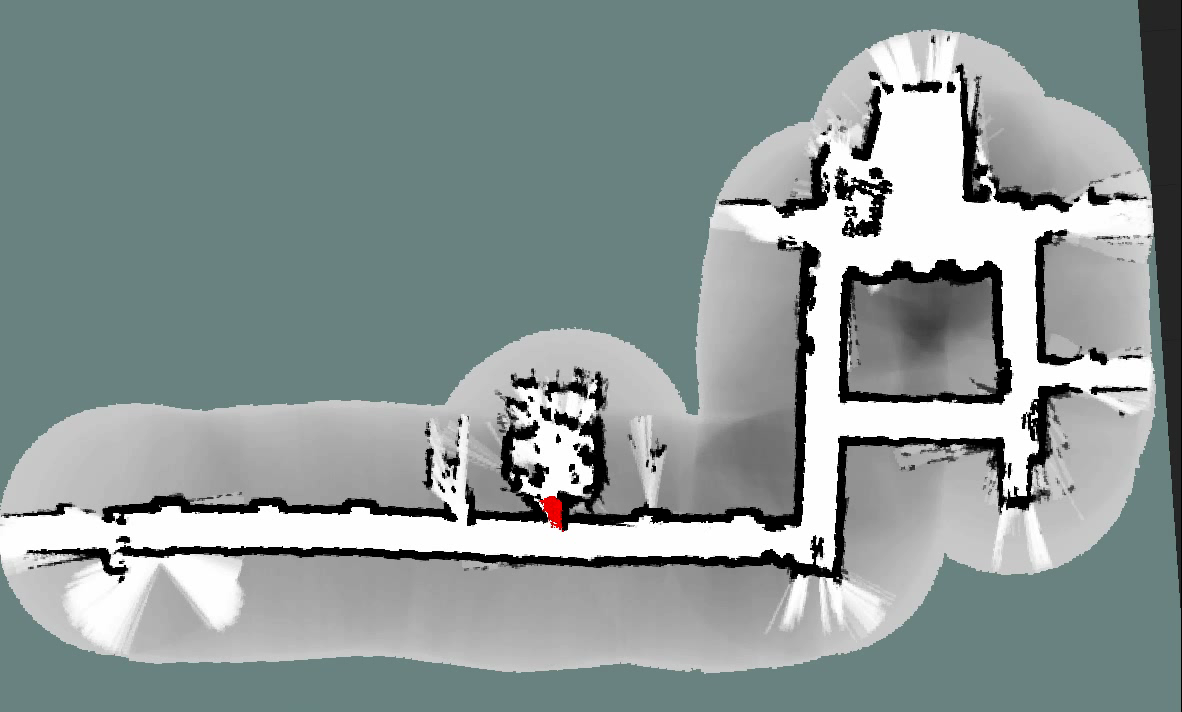
\includegraphics[width=\linewidth]{figures/Screenshot-video_log1-10k_good-4}
\caption{Particles finish inside the room, as expected}
\label{fig:Screenshot-video_log1-10k_good-4}
\end{subfigure}
\caption{Snapshots from \texttt{robotdata1.log} showing particles converging to the long hallway, turning around at the end, and entering the room.
\label{fig:Screenshot-video_log1-10k_good}}
\end{figure}



\subsection{Dataset 2: \texttt{ascii-robotdata5.log}}

Figure~\ref{fig:Screenshot-video_log5-10k_goodenough} shows a few snapshots from a run using the fifth data log. Again, the particles converge to one cluster reasonably quickly and traverse the hallway. However, we noticed the cluster seems to overshoot when making the turn, leading to many particles being constrained by the wall, and consequently down-weighted. This problem seems to resolve itself though, as the particles are able to complete the turn. Though there was no ground truth provided for this set, the motion of the final cluster of particles seems to be consistent with the odometry data (Fig.~\ref{fig:log5odom}). Total runtime was around 35 minutes.\\
Video is available here:  \url{https://www.youtube.com/watch?v=AgGZ6cR-dyk}


\begin{figure}
\centering
\begin{subfigure}[b]{0.49\textwidth}
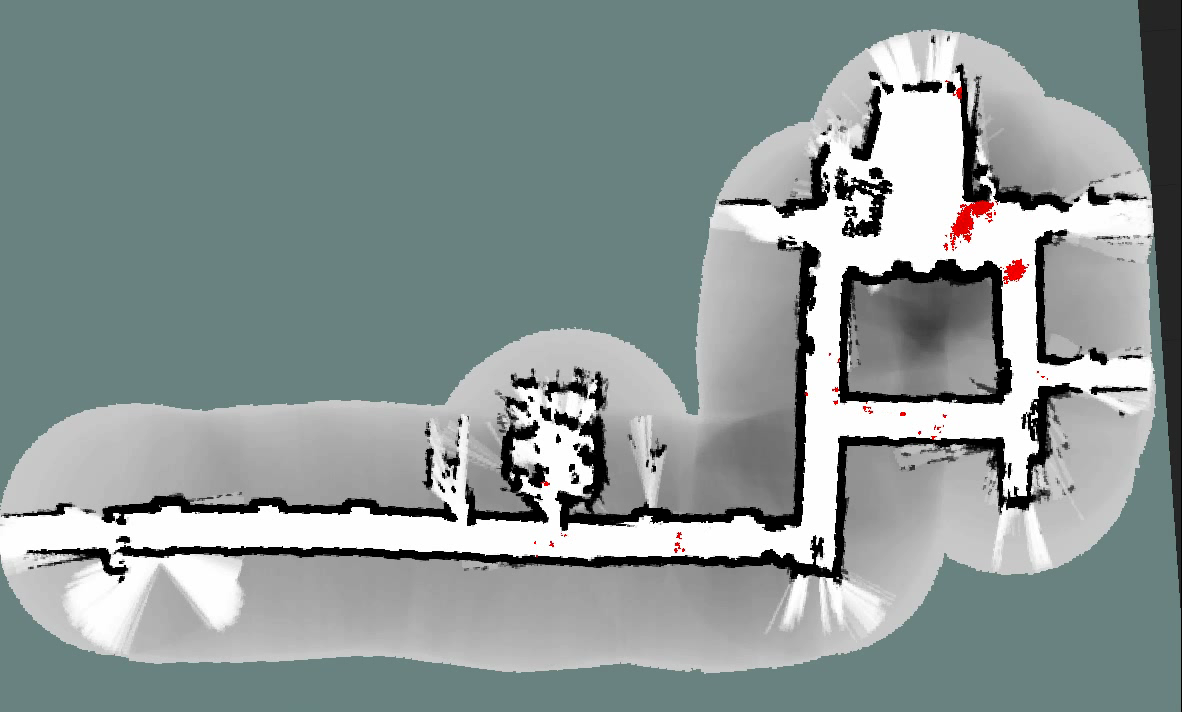
\includegraphics[width=\linewidth]{figures/Screenshot-video_log5-10k_goodenough-1}
\caption{Particles start converging to two large clusters}
\label{fig:Screenshot-video_log5-10k_goodenough-1}
\end{subfigure}
\begin{subfigure}[b]{0.49\textwidth}
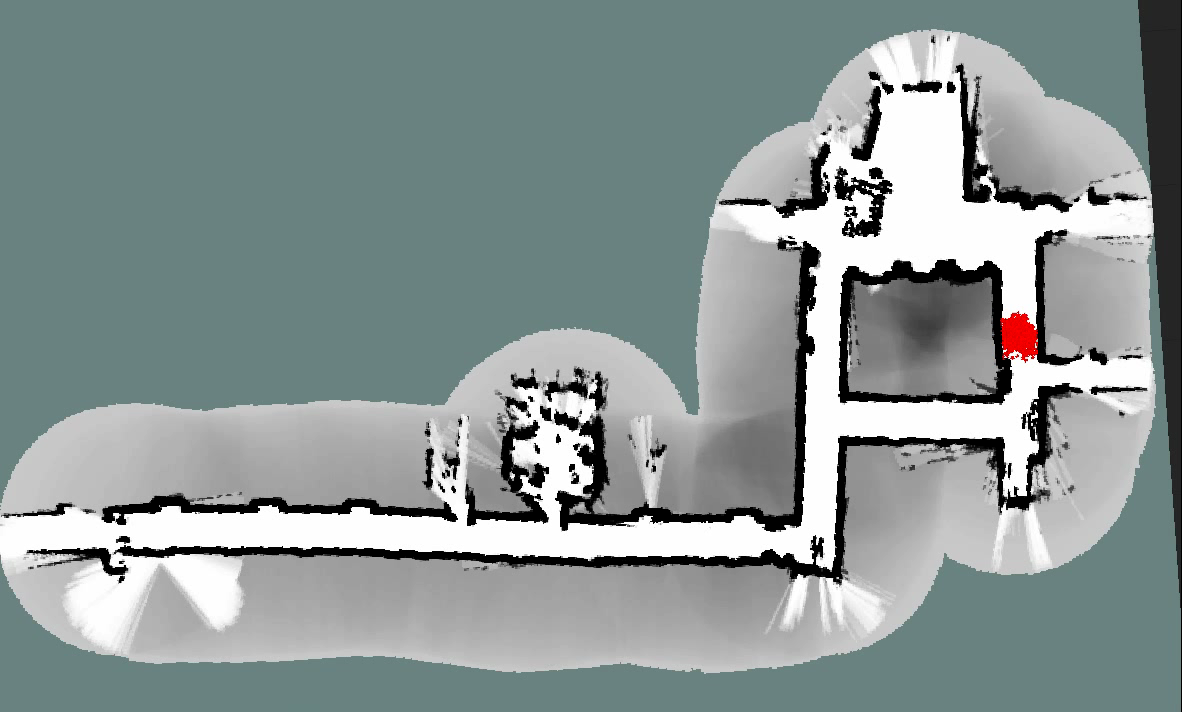
\includegraphics[width=\linewidth]{figures/Screenshot-video_log5-10k_goodenough-2}
\caption{Second cluster dominates}
\label{fig:Screenshot-video_log5-10k_goodenough-2}
\end{subfigure}
\\
\begin{subfigure}[b]{0.49\textwidth}
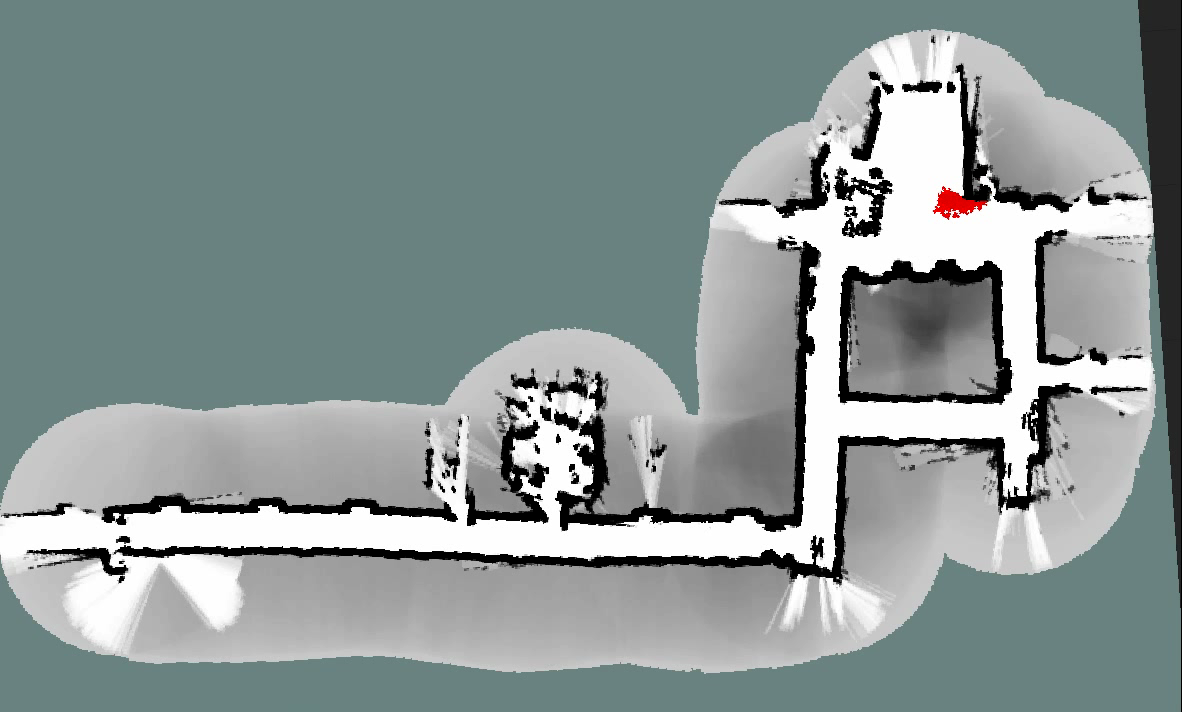
\includegraphics[width=\linewidth]{figures/Screenshot-video_log5-10k_goodenough-3}
\caption{Particles turning left into the open area but seem slightly off}
\label{fig:Screenshot-video_log5-10k_goodenough-3}
\end{subfigure}
\begin{subfigure}[b]{0.49\textwidth}
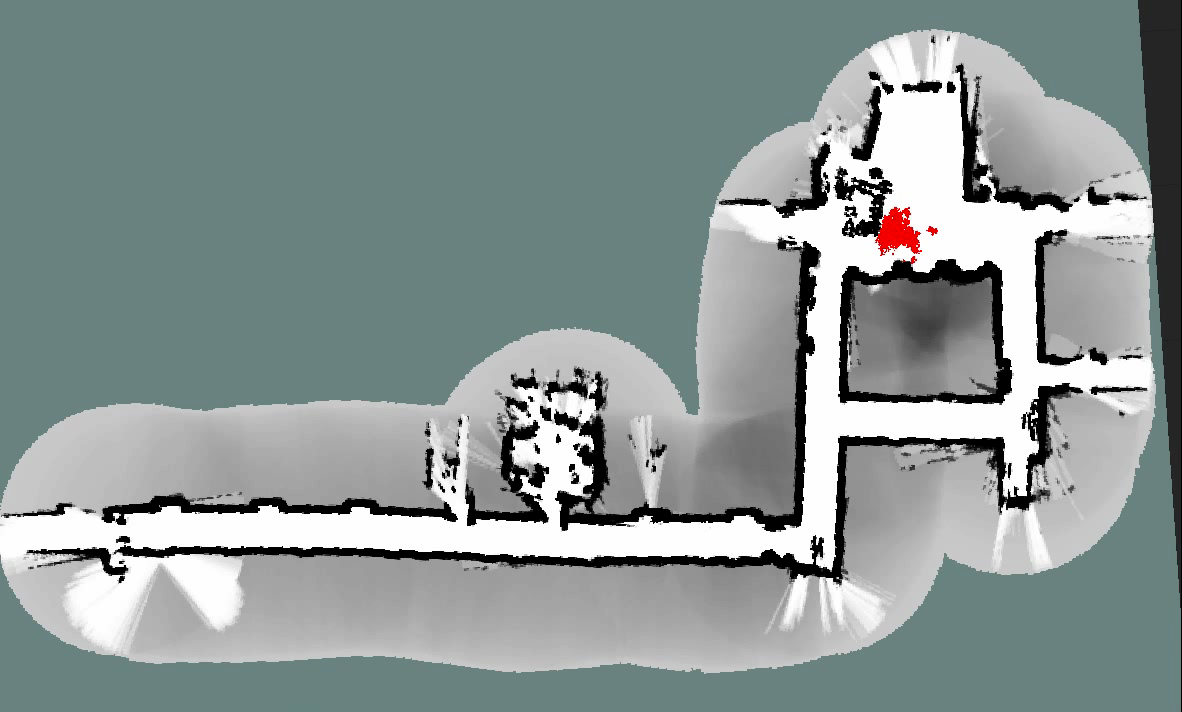
\includegraphics[width=\linewidth]{figures/Screenshot-video_log5-10k_goodenough-4}
\caption{Particles complete the left turn and stop}
\label{fig:Screenshot-video_log5-10k_goodenough-4}
\end{subfigure}
\caption{Snapshots from \texttt{ascii-robotdata5.log} showing particles converging to the hallway on the right, turning around partway through, and turning left into the open area at the top.
\label{fig:Screenshot-video_log5-10k_goodenough}}
\end{figure}

\begin{figure}
\centering
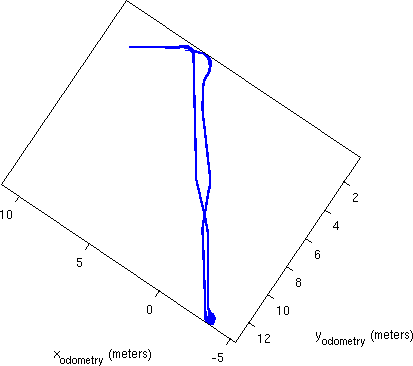
\includegraphics[width=0.45\linewidth]{figures/log5odom}
\caption{Odometry data from \texttt{ascii-robotdata5.log}}
\label{fig:log5odom}
\end{figure}


\section{Future Work}

One obvious extension to our approach would be to use the laser range return model from Probabilistic Robotics.
In Section \ref{sec:sensor_model}, we only modeled $P_\text{hit}$.
This should be extended to include models for dynamic obstacles, random noise, and max range sensor failures.

\bibliography{refs}

\end{document}
